%-------
% Gayatri Belapurkar's resume.
%-------

%-------
% Basic configurations for the document. This resume makes use of the res.cls template, a copy of which can be found 
% on https://rpi.edu/dept/arc/training/latex/resumes/ 
%-------
\documentclass[margin]{res}
\textwidth=5.2in 
            		 
% Use pdf, png, jpg, or eps§ with pdflatex; use eps in DVI mode
\usepackage{graphicx}														

\begin{document}

%---
% Defining new command for superscript usage
%---
\newcommand{\ts}{\textsuperscript} 

%----
% Basic details 
%----
\name{Gayatri Vyankatesh Belapurkar\\[13pt]}
\address{{\bf Address} \\91 A, Kamgar Nagar \\ Kurla East \\ Mumbai 400024}
\address{{\bf Contact Details} \\Mob: +91-9920697529 \\ Email: gayatri.belapurkar5@gmail.com}

\begin{resume}

%----
% Photo
%----
\begin{figure}[h!]
    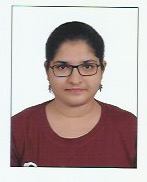
\includegraphics[scale=0.5]{Photo_gayatri.jpeg}
\end{figure}

%----
% Section: Objective
%----
\section{Objective}
Seeking a summer internship at Department of Computer Science and Engineering, IIT-Bombay under the e-Yantra Summer Internship program. 

%----
% Section: Education
%----
\section{Education}
\begin{table}[h!]
  \begin{tabular}{p{0.5cm}|p{4cm}|p{3.5cm}|p{2cm}|p{1.5cm}|p{1.6cm}}
    \textbf{Sr.} & \textbf{Degree} & \textbf{College} & \textbf{University} & \textbf{Passing Year} & \textbf{Pass Percentage} \\
    \hline
    1. & B.E., Information Technology. & Vivekanand Education Society's Institute of Technology. & University of Mumbai. & 2020 & 8.94\\
    2. & XII\ts{th} Higher Secondary Certificate. & Swami Vivekanand Junior College. & Maharashtra State Board. & 2016 & 84\%\\
    3. & X\ts{th }C.B.S.E. & Atomic Energy Central School-6. & Central Board of Secondary Education. & 2012 &  97.6\%\\
    \end{tabular}
\end{table}

%----
% Section: Projects
%----
\section{Projects}
\begin{enumerate}
  \item {\bf Smart Subsidy System using blockchain}
  
  Enter a meaningful description here. 
  \item {\bf IoT based Street Quality Identification using 'Z-algorithm' }
  
  Enter a meaningful description here. 
  \item {\bf IoT based detection of public toilet usage and incentivization}
  
  Enter a meaningful description here. 
  \item {\bf Asset Management System}
  
  Enter meaningful description here.
  \item {\bf Blockchain and web development}
  
  Enter a meaningful title and description here.
  \item {\bf App for converting text in images from English to a different language}
\end{enumerate}

  %----
  % Internship
  %----
  \section{Internships}
  \begin{itemize}
    \item {\bf Software Development Internship},  AppStack \hfill Jun 2018 - Oct 2018
    
    Worked as an intern with AppStack for Android and iOS application development using React Native. 
    \item {\bf Winter Internship}, VESIT \hfill Dec 2017 - Jan 2018
    
    Worked as an intern on developing staff attendance module in VESIT Content Management System, focusing primarily on 
    attendance synchronization and data transfer.
    
 \end{itemize}
 
%----
% Research Publications
%----
\section{Research Publication}
\begin{enumerate}
  \item None. 
\end{enumerate}

%----
% Technical Skills
%----
\section{Technical Skills}
\begin{itemize}
  \item Programming Languages: C, C++, Java, Python
  \item App Development using React Native and Ionic
  \item Web development using HTMP, CSS, PHP, Laravel framework
  \item Data mining and database management
  \item Basics of Machine Learning
\end{itemize}

%----
% Soft Skills
%----
\section{Soft Skills}
\begin{enumerate}
  \item Team leader and team player
  \item Responsible
  \item Efficient communicator
  \item Rational and logical perspective
  \item Problem solving and conflict resolution
\end{enumerate}

%----
% Extra Curricular Activities
%----
\section{Extra Curricular Activities}
\begin{itemize}
  \item {\bf Student Chief Editor}, VESIT Connect \hfill Apr 2018 - Present
  
  Currently working as the Student Chief Editor of VESIT Connect (monthly newsletter) and of Vishwakarma (annual magazine)  of Vivekanand Education Society's Institute of Technology. 
  \item {\bf VESIT Badminton team} \hfill Sep 2018 - Present
  \item {\bf Student Reporter}, VESIT Connect \hfill Jul 2017 - Mar 2018
  \item {\bf Technical Assistance Team}, Praxis \hfill Sep 2017
  \item {\bf Aesthetic team}, Illusions \hfill Jan 2017
\end{itemize}

%----
% Co-Curricular Activities
%----
\section{Co-Curricular Activities}
\begin{enumerate}
\item Workshops \#1
\item Workshops \#2
\end{enumerate}

%----
% Achievements
%----
\section{Achievements}
\begin{itemize}
\item Winner of Smart India Hackathon, 2019
\item Winner in 'Best Algorithm' category in e-Yantra Ideas Competition, 2019
\item Semi-finalist in Project Deep Blue, 2019
\item Winner of hackathon 'VESIT Hacks' held in Praxis 2018
\item Top 25 teams in ACM Women's Hackathon. 
\item Won multiple events in VESIT cultural festival - Utsav in 2018 (2\ts{nd} in Drama, 2\ts{nd} in Rangoli, 2\ts{nd} in Paper Dressing, 3\ts{rd} in Tshirt Painting and Nail art)
\item Semi-finalist in inter-college Badminton Competition (women's doubles) in Skream, the Annual Sports Festival organized by K.J. Somaiya College.
\item Quarter-finalist in inter-college Badminton Competition (women's singles) in Skream, the Annual Sports Festival organized by K.J. Somaiya College.
\end{itemize}

%----
% Personal Information
%----
\section{Personal Information}
Father's Name: Vyankatesh Chandrakant Belapurkar

Mother's Name: Manisha Vyankatesh Belapurkar

Sex: Female

Date of Birth: 25/11/1998

Nationality: Indian

Marital Status: Single

\end{resume}

\end{document}  